\section{Empirical Determination of Comparison Operations}

We empirically determine the number of comparisons between array elements for large, randomly generated arrays.
For Shellsort, we expect the runtime complexity to lie between $O(n\ \lg\ n)$ and $O(n^2)$.
To count the number of element comparisons, a counting variable $c_3$ can be employed, as illustrated in Listing~\ref{lst:shell}.
This variable increments each time an element comparison is performed.
Random arrays can be generated according to the method shown in Listing~\ref{lst:rand}, and the observed values of $c_3$ are recorded.
Since every comparison-based sorting algorithm belongs to the complexity class $\Omega(n\ \lg\ n)$, it is reasonable to assume that, on average, $c_3 \geq n\ \lg\ n$ holds (\cite[154]{OW17b}).\\

Early \textit{empirical} findings led \textit{Shell} to the assumption:\\

\blockquote[{\cite[31]{She59}}]{It appears that the time required to sort $n$ elements is proportional to $n^{1.226}$.
}\\

Naturally, these tests were constrained by small input sizes and the performance limitations of late 1950s hardware.
To avoid misinterpretations regarding the asymptotic upper bound of $O(n \log n)$, it is important to examine its growth behavior for varying $n$.
Notably, the inequality $n^{\frac{4}{3}} > n \log n$ holds for input sizes $n \geq 982$ (see Figure~\ref{fig:lognplot}).

\begin{figure}[!h]
    \centering
    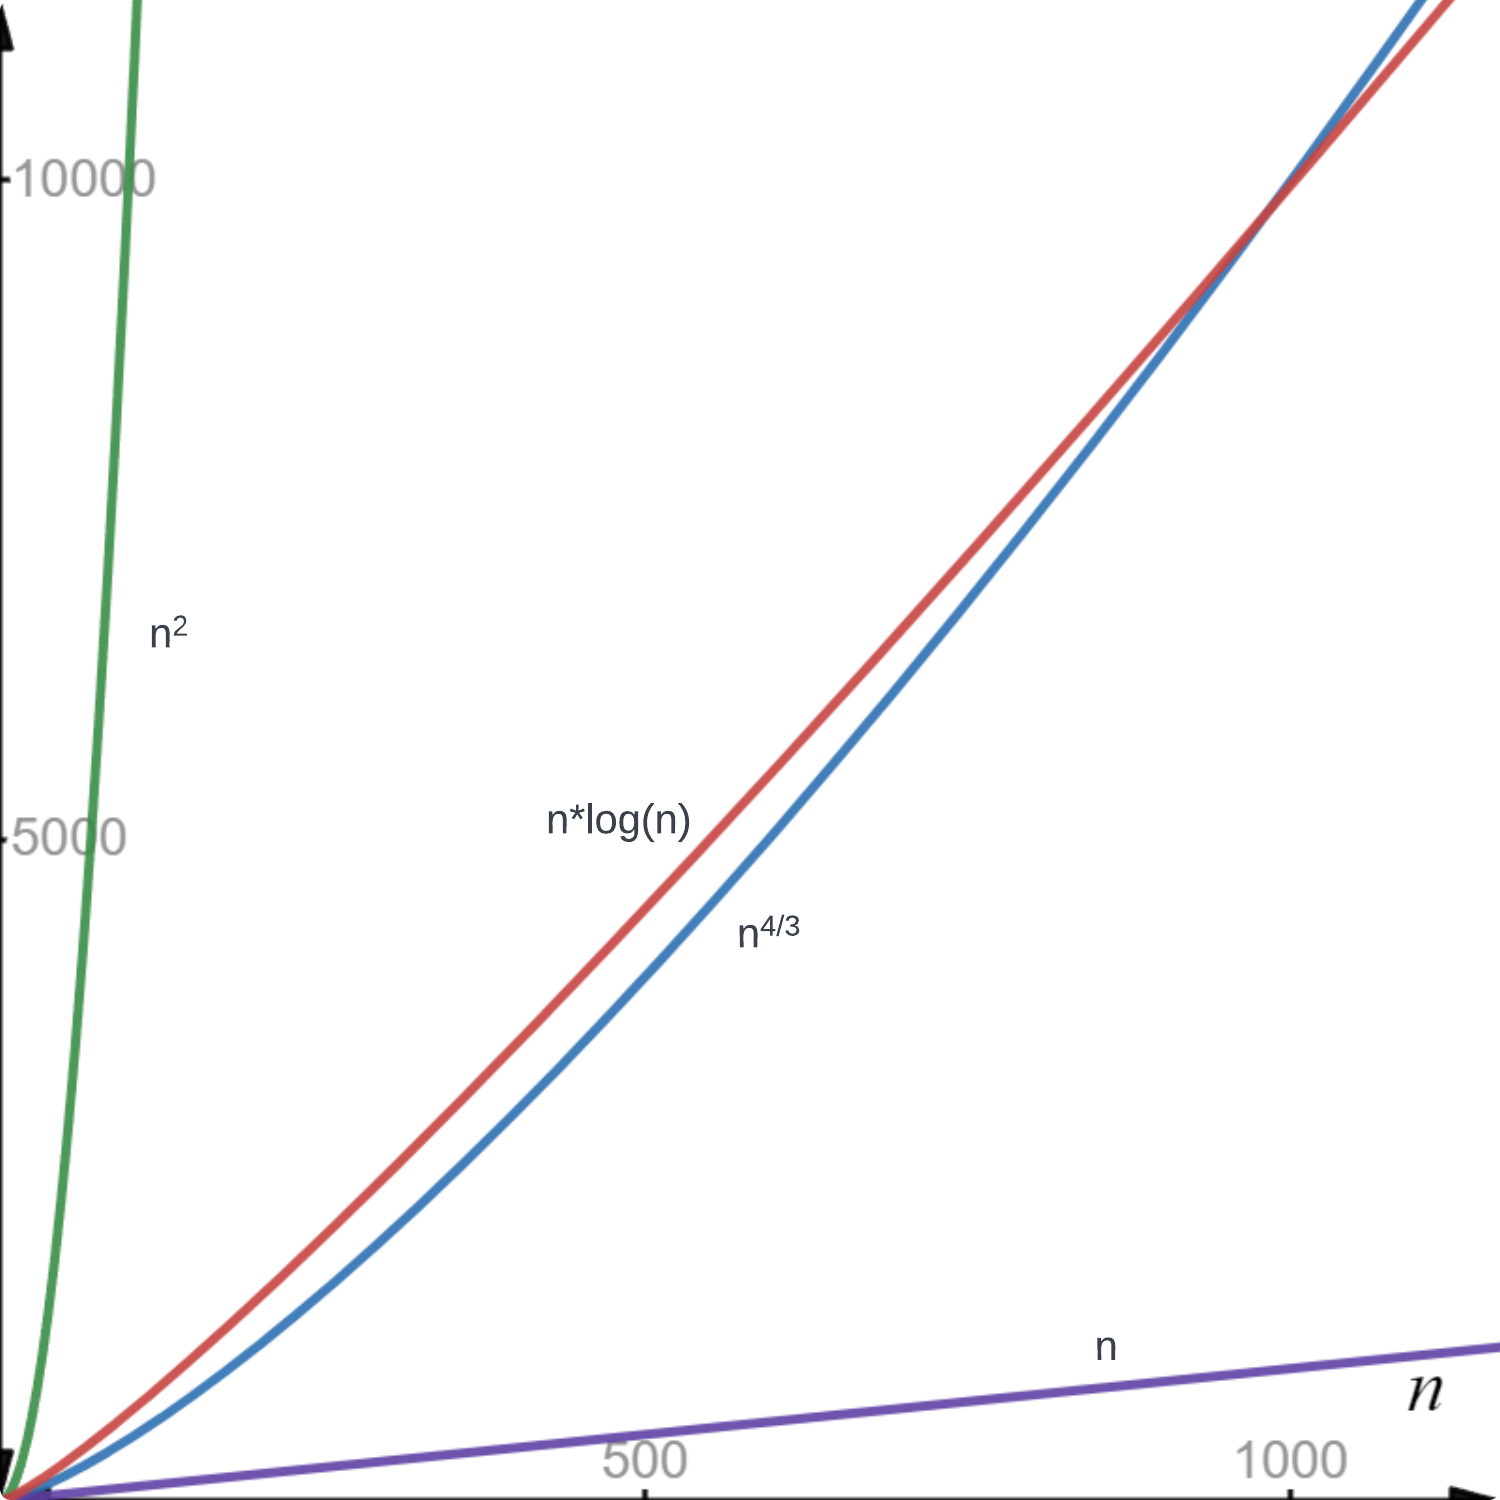
\includegraphics[width=1\columnwidth]{img/lognplot}
    \caption{For $n \geq 982$, $n^{\frac{4}{3}}$ grows faster than $n \log n$.}
    \label{fig:lognplot}
\end{figure}

\noindent
This behavior must be carefully considered when interpreting empirical results for $n$.
Otherwise, one might incorrectly conclude that Shellsort achieves optimal runtime complexity of $O(n \log n)$, while in fact the observed upper bound of $O(n^{4/3})$ already exceeds $n \log n$ and approaches quadratic complexity for larger $n$.



\vspace{4mm}
\begin{lstlisting}[style=javastyle, caption={Code for Shellsort-testing large randomized arrays.}, label=lst:rand]
int epochs = 1000;
int bound  = 2_000_000;
while(epochs-- > 0) {
    Random r = new Random(epochs);
    int[] arr = new int[bound];

    for (int i = 0; i < bound; i++) {
        arr[i] = r.nextInt(bound + 1);
    }

    ShellSort.sort(
        Arrays.copyOfRange(
            arr, 0, arr.length));
}
\end{lstlisting}
\vspace{4mm}


\subsection{Test Results}
Shellsort demonstrates remarkable stability in empirical tests, confirming early observations made by \textit{Shell}.
For larger input sizes (up to $n = 2.000.000$; see Listing~\ref{lst:rand}), our empirical measurements consistently yielded comparison counts $c_3$ below an upper bound of $O(n^{1.3})$  ($< O(n^{\frac{4}{3}})$).
Interestingly, none of our test runs was below a bound of $O(n^{1.27})$.

\noindent
These results support the hypothesis that Shellsort, when using the classical halving sequence originally proposed by \textit{Shell}, exhibits sub-quadratic runtime behavior on average.
